\label{gaps} 

It is a curious fact that many constraints on underlying representations are elegantly described using the units of prosody.
In some cases, these are part of the system of contrast, such as long segments in moraic theory \citep[e.g.,][]{Davis1999}. For instance, Latin has constrastive consonant and vowel length (e.g., \emph{anus} `ring' vs.~\emph{annus} `year', \emph{os} `bone' vs.~\emph{ōs} `mouth'), but there is no vowel length contrast before geminate consonants. However, constraints on underlying representations may also involve references to non-contrastive prosodic structures, such as syllables (e.g., \citealt{Hooper1973}, \citealt{Kahn1976}).\footnote{See \citealt{Blevins1995} for the claim that syllable structure is universally non-contrastive, and \citealt{Elfner2006} for arguments that a putative counterexample is the result of an underlying moraic, not syllabic, contrast.}
For instance, as \citeauthor{Haugen1956} first notes, the constraints on word-medial consonant clusters are not arbitrary in prosodic terms:

\begin{example}[\textsc{Medial Cluster Law} (after \citealt{Haugen1956})]
\label{mcl}
A medial cluster must consist of a well-formed medial coda and a well-formed medial onset
\end{example}

\noindent
It is not necessary for predictable prosodic structure to be present in underlying form to achieve this effect, contrary to what has sometimes been stated \citep[e.g.,][255]{A74}.
All that is necesary is that no phonological processes intervene between underlying representation and the surface form of medial clusters.
Under the further assumption that underlying and surface representations are as similar as alternations allow (e.g., \citealt[205f.]{Dell1973}, \citealt[28f.]{Stampe1973}), this is the null hypothesis. 

In a study of English word-medial consonant clusters, \citet{Pierrehumbert1994} notes that the vast majority of ``possible clusters'', those which can be parsed into coda and onset in accordance with the \textsc{Medial Cluster Law}, are unattested.
\citeauthor{Pierrehumbert1994} argues that this can be accounted for by positing static co-occurrence restrictions---unrelated to any phonological alternation in English.
This study argues that well-known phonological processes, but not the static constraints proposed by \citeauthor{Pierrehumbert1994}, impose restrictions on this inventory.
%\citeauthor{Pierrehumbert1994}'s static constraints are not statistically valid

\section{English syllable contact clusters}

English syllable contact clusters have been used, by \citeauthor{Pierrehumbert1994} and others, to argue for the necessity of admitting static phonotactic constraints, and to illustrate proposals for the architecture of the phonotactic system. 
However, there are a number of reasons to reconsider the facts of this domain.

\subsection{The role of phonological processes}

\citeauthor{Pierrehumbert1994} does not fully consider the effects of phonological processes targeting word-medial clusters in English, and consequently some of the static constraints she proposes may be related to English morphophonemics. 
For instance, she writes that ``nasal-stop sequences agree in labiality'' (175), and attributes this the status of a static constraint. 
However, this generalization is just a narrower form of the one derived by \textsc{Nasal Place Assimilation} (see \S\ref{npa}), and which requires no further explanation. 
Other derived constraints go unnoticed: for instance, she does not discuss the highly reliable tendency of obstruent-obstruent clusters to agree in voicing (see \S\ref{ova}). 
The evaluation below considers the role of both types of constraints on the English lexicon on an equal footing.

\subsection{The role of sparsity}

\citet{Pierrehumbert1994} infers static constraints from near-exceptionless gaps in the lexicon, but little effort is made to show that the patterns of lexical underrepresentation are not due to chance. 
Consquently, it is possible to suggest that some of these gaps 
are accidental rather than structural in nature.
%\citep{Fischer-Jorgensen1952,Vogt1954}. 
This is made all the more likely given the tendency of segment and cluster frequency distributions to be highly skewed \citep[e.g.,][]{Pande2010,Sigurd1968,Tambovtsev2007,Weiss1961}. 
Furthermore, \citeauthor{Pierrehumbert1994} considers only triconsonantal clusters, but medial clusters may be as short as two consonants, as in \emph{a}[n.t]\emph{ics}, or as long as four, as in \emph{mi}[n.str]\emph{el}, and \citeauthor{Pierrehumbert1994} offers no justification for a narrower focus.
If this has any effect on the distribution of clusters, it would be to impose further sparsity.

\subsection{The role of morphological segmentation}

Many components of \citeauthor{Pierrehumbert1994}'s study cannot be directly replicated. \citeauthor{Pierrehumbert1994} focuses her attention on those words she judges to be ``morphologically simple'' and ``reasonably familiar'', but this list has neither been published nor circulated.
It is not clear that the judgements (as well as cognitive limitations) of concerned parties should be granted evidential status in the first place, given the potential for implicit bias; 
\citet{Labov1975}, for instance
argues for what he calls the \emph{Experimenter Principle}, 
that the intuitions of all those familiar with the formal matters should be excluded.
Otherwise-unmotivated morphological junctures are sometimes posited simply to preserve phonological or phonotactic generalizations; 
%The same practice is sometimes applied to preserve phonological generalizations; for instance, otherwise unmotivated morphological boundaries are used in \emph{SPE} to simplify principles of stress assignment. 
this is done by \citet{SPE}, for instance, to simplify principles of English stress assignment, and \citet[546]{Rice2009d} analyses many words in Slave as compounds simply because they contain consonant clusters that rarely occur morph-internally. 
%There is some evidence that infants \citep{Mattys2001b} and adults \citep{Brown1956,Hay2004a,McQueen1998b,Norris1997} use this heuristic to segment fluent speech in experimental settings. 
Applied indiscriminately, however, such a heuristic trivializes both morphological segmentation and phonotactic generalization.
For these reasons, the wordlist used in this study is derived from a publicly available database, and no experimenter intuitions are used for establishing morphological boundaries.

%Such reasoning is found in \citeauthor{Pierrehumbert1994}'s discussion of the word \emph{a}[nt.l]\emph{er}, however: this contains a cluster which violates her constraint on coda coronal obstruents, and therefore must be a complex word, she argues (see \citealt[164]{Borowsky1989} for additional exceptions to this generalization).

\section{Evaluation}
\label{4evaluation}

After constructing a sample of syllable contact clusters in English simplex words, this data is used to evaluate the coverage of static and phonologically derived constraints.

\subsection{Method}

\subsubsection{Materials and procedure}

Following \citet[ chap.~8]{Duanmu2009} and \citet[ chap.~3]{Hammond1999a}, 
a wordlist is generated using the English portion of the CELEX database \citep{CELEX}. 
Only words coded as ``monomorphemic'' are used, and all words coded as non-native are excluded.
This stringent criterion for inclusion eliminates many of the exceptions noted by \citeauthor{Duanmu2009} or \citeauthor{Hammond1999a} in their studies. For instance, nearly all the exceptions to \textsc{Obstruent Voice Assimilation} (see \S\ref{ova} below) noted by \citet[74]{Hammond1999a} are 
either complex words (e.g., \emph{jurisdiction}, \emph{madcap} \emph{tadpole}, \emph{scapegoat}, \emph{magpie}) or non-native (e.g., \emph{vodka}, \emph{smorgasbord}).

Unlike prior studies, however, words which appear to consist of a Latinate prefix and a bound stem (e.g., \emph{inspect}, \emph{excrete}) are also excluded from the sample, as there is broad formal and experimental support for the claim that these words are complex.
This assumption allows for numerous simplifications to accounts of the phonological shape of these forms. 
For instance, \citet[11f.]{Aronoff1976} observes that Latinate forms which share the same bound stem also share irregular allomorphs of that stem under derivation. 

\begin{example}[Bound stem-specific allomorphy]
\begin{tabular}{l l l l l l}
a. & {adhere}   & {adhesion}   \\
   & {cohere}   & {cohesion}   \\
b. & {conceive} & {conception} \\
   & {perceive} & {perception} \\
\end{tabular}
\end{example}

\noindent
\citeauthor{Aronoff1976} takes this to be evidence that \emph{adhere} and \emph{cohere}, for instance, share a bound stem.
There is also an interaction between Latinate prefixes on verbs and the makeup of the verbal complement. 
Latinate verbs do not generally allow ditransitive, verb participle, or adjectival resultative constructions, all acceptable with similar Anglo-Saxon verbs \citep{Gropen1989,Harley2009}.
%\citep[see also][]{Gropen1989,Coppock2008}. 

\begin{example}[Latinate verbs and small clauses] 
\label{harley}
\begin{tabular}{l l l l@{} l}
a. & {show him the painting} & \alt{} & * & {exhibit him the painting} \\
b. & {drink himself stupid}  & \alt{} & * & {imbibe himself stupid}    \\
c. & {show it off}           & \alt{} & * & {exhibit it off}           \\
\end{tabular}
\end{example}

Lexical decision experiments also suggest that Latinate prefixed forms are complex. \citet{Taft1975,Taft1976} and \citet{Taft1986} find that nonce words like \emph{*re-sert}, which appear to be composed of a prefix and a bound stem, take longer to reject that non-words which lack apparent morphological structure, such as *\emph{refant}. 
Bound stems also show frequency effects which are independent of whole word frequency \citep{Taft1979,Taft2006}. 
Finally, \citet{Emmorey1989} and \citet{Forster2000} report facilitative priming between pairs like \emph{permit}-\emph{submit}, an effect thought to indicate morphological relatedness.

\subsection{Results}

This results in a list of 6,619 simplex words. 
The full set of clusters and their frequencies are given in Appendix \ref{clusters}.
The CELEX transcriptions of these words were then syllabified and phonologized using a technique described in Appendix \ref{syllabification}. 
This produces 23 unique medial codas and 40 unique medial onsets. 
Of the 920 ($= 21 \times 40$) medial clusters that would result from free combination, 174 (19\%) are attested. 

\subsubsection{Static constraints}

So as to account for the 81\% of ``possible'' but unattested clusters, \citet{Pierrehumbert1994} proposes three constraints on English medial clusters. These constraints are static, in the sense that they have no analogues in the morphophonemics of English.

\paragraph{Dorsal-labial clusters} 
\citet[173]{Pierrehumbert1994} writes that ``velar obstruents occurred only before coronals in the clusters studied, never before labials or other velars'', noting that velar-velar clusters are independently excluded by constraints on geminates (see \S?). 
Two-consonant velar-labial clusters are found in words like \emph{a}[k.m]\emph{e}, \emph{ru}[ɡ.b]\emph{y}, or \emph{pi}[ɡ.m]\emph{ent} occur. 
Table \ref{dltab} shows that velar-labial clusters are somewhat less likely to occur than  are velar-coronal clusters (e.g., \emph{ve}[k.t]\emph{or}), but such underrepresentation is not unlikely to occur by chance ($p = .106$).

\begin{table}
\centering
\begin{tabular}{l rrrr}
\toprule
           & attested & unattested & saturation & $p$-value \\
\midrule
conforming & 25       & 91         & 22\%       & \multirow{2}{*}{.106} \\
violating  &  4       & 40         &  9\%       \\
\bottomrule
\end{tabular}
\caption{Dorsal-labial cluster attestation in the lexical sample}
\label{dltab}
\end{table}

\paragraph{Coronal obstruent codas} 
\citet[175]{Pierrehumbert1994} claims that ``clusters with a coronal obstruent in the coda do not occur'', while noting exceptions like \emph{a}[nt.l]\emph{er}, \emph{ke}[s.tr]\emph{el} and \emph{oi}[nt.m]\emph{ent}. 
Table \ref{cctab} reveals that coda coronal obstruent clusters are not significantly less likely to occur than non-coronal obstruent clusters (e.g., \emph{re}[p.t]\emph{ile}). 
The same is true if attention is restricted to triconsonantal clusters ($p = .129$).

\begin{table}
\centering
\begin{tabular}{l rrrr}
\toprule
           & attested & unattested & saturation & $p$-value \\
\midrule
conforming & 56       & 304        & 15\%       & \multirow{2}{*}{.430} \\
violating  & 37       & 243        & 13\%       \\
\bottomrule
\end{tabular}
\caption{Coda coronal obstruent cluster attestation in the lexical sample}
\label{cctab}
\end{table}

\paragraph{ABA clusters} 
\citet[176]{Pierrehumbert1994} notes the ``lack of clusters with identical first and third elements'', ignoring presence or absence of voicing. 
Despite the fact that there are no exceptions to this generalization, these \textsc{ABA} clusters are not significantly less common than other triconsonantal and quadraconsonantal clusters (Table \ref{abatab}).

\begin{table}
\centering
\begin{tabular}{l rrrr}
\toprule
           & attested & unattested & saturation & $p$-value \\
\midrule
conforming & 47       & 512        &  8\%       & \multirow{2}{*}{.250} \\
violating  &  0       &  25        &  0\%       \\
\bottomrule
\end{tabular}
\caption{ABA cluster attestation in the lexical sample}
\label{abatab}
\end{table}

\paragraph{Summary} 
There is no statistical support for \citeauthor{Pierrehumbert1994}'s static constraints.

\subsubsection{Derived constraints}

In \emph{The Sound Pattern of English} (henceforth, \emph{SPE}), \citet{SPE} describe three phonological processes which target medial consonant clusters. As will be shown, the neutralizing effect of these three processes has a major influence on the cluster inventory.

\paragraph{Obstruent voice assimilation}
\label{ova}

Voice assimilation alternations are evidenced by the non-syllabic allomorphs of the regular past (e.g., \emph{nap}[t] $\sim$ \emph{nab}[d]) and noun plural (e.g., \emph{lap}[s] $\sim$ \emph{lab}[z]), which take the voicing specification of a preceding obstruent.\footnote{Underlying /-d, -z/ are assumed here (e.g., \citealt{Anderson1973a}, \citealt[284f.]{Bakovic2005b}, \citealt{Basboll1972}, \citealt[210]{SPE}, \citealt[282]{Hockett1958}, \citealt[102]{Pinker1988}, \citealt{Shibatani1972}); alternative analyses are put forth by \citet[210f.]{LANGUAGE}, \citet[135]{Borowsky1986}, \citet{Hoard1971}, \citet{Kiparsky1985}, \citet{Lightner1970}, \citet{Luelsdorff1969}, \citet{Miner1975}, \citet[426]{Nida1948}, and \citet{Zwicky1975}.}
%Bizarely, \citet[208]{Wetzels2001}, cite English as an example of a language without ``general devoicing or assimilatory effects''. 

\begin{example}[\textsc{Obstruent Voice Assimilation}]
\label{ovarule}
$\begin{bmatrix} -\textsc{Son} \end{bmatrix}~\goesto~\begin{bmatrix} =\textsc{Voi} \end{bmatrix}~/~\gap~\begin{bmatrix} =\textsc{Voi} \\ -\textsc{Son} \end{bmatrix}$
\end{example}

\noindent
\citet{Pierrehumbert1994} does not discuss a constraint against adjacent obstruents disagreeing in voice. 
As shown in Table \ref{ovatab} however, the vast majority of medial obstruents clusters in simplex words are either uniformly voiced, as in \emph{hu}[z.b]\emph{and}, or uniformly voiceless, as in or \emph{rha}[p.s]\emph{osdy}. Hetero-voiced clusters, like those in \emph{a}[b.s]\emph{inth} and \emph{a}[s.b]\emph{estos}, are rarer than would be expected from chance.

\begin{table}
\centering
\begin{tabular}{l rrrr}
\toprule
           & attested & unattested & saturation & $p$-value \\
\midrule
conforming & 35       & 329        & 10\%       & \multirow{2}{*}{.002} \\
violating  & 11       & 305        &  3\%       \\
\bottomrule
\end{tabular}
\caption{Obstruent voice assimilation cluster attestation in the lexical sample}
\label{ovatab}
\end{table}

\paragraph{Nasal place assimilation}
\label{npa}

\textsc{Nasal Place Assimilation} (e.g., \citealt[65f.]{Borowsky1986}, \emph{SPE}:85, \citealt[62]{Halle1985a}) permits [ŋ] to be described as a pure allophone of /n/, and accounts for certain patterns in Latinate prefix allomorphy.

\begin{example}[\emph{im-}/\emph{in-} allomorphy]
\label{nparule}
\begin{tabular}{l l l l l l l}
a. & {polite}   & {i}[m.p]{olite}   \\
   & {balance}  & {i}[m.b]{alance}  \\
b. & {tangible} & {i}[n.t]{angible} \\
   & {decent}   & {i}[n.d]{ecent}   \\
\end{tabular}
\end{example}

%Furthermore, \citet[228]{Myers1993} reports speech errors which create nasal-obstruent clusters and undergo \textsc{Nasal Place Assimilation}; e.g., \emph{ra}[nd] \emph{orker}, intended \emph{ra}[ŋk] \emph{order}. 

\noindent
The rule is formalized below.

\begin{example}[\textsc{Nasal Place Assimilation}]
$\begin{bmatrix} $+$\textsc{Nas} \end{bmatrix}~\goesto~\begin{bmatrix} =\textsc{Lab} \\ =\textsc{Cor} \\ =\textsc{Dor} \end{bmatrix}~/~\gap{}~\begin{bmatrix} =\textsc{Lab} \\ =\textsc{Cor} \\ =\textsc{Dor} \\ -\textsc{Son} \end{bmatrix}$
\end{example}

\noindent
As shown in Table \ref{npatab}, virtually all clusters consisting of a nasal coda followed by a homorganic obstruent (e.g., \emph{pi}[m.p]\emph{le}, \emph{sta}[n.z]\emph{a}, \emph{mo}[ŋ.k]\emph{ey}) are attested. As \citet[175]{Pierrehumbert1994} observes, heterorganic clusters, like those \emph{pli}[m.s]\emph{oll} or \emph{scri}[m.ʃ]\emph{aw}, do occur, but they are significantly more rare.

\begin{table}
\centering
\begin{tabular}{l rrrr}
\toprule
           & attested & unattested & saturation & $p$-value \\
\midrule
conforming & 31       & 2          & 94\%       & \multirow{2}{*}{3.4\e{-07}} \\
violating  & 11       & 22         & 33\%       \\
\bottomrule
\end{tabular}
\caption{Nasal place assimilation cluster attestation in the lexical sample}
\label{npatab}
\end{table}

\paragraph{Degemination} The final alternation found in English medial clusters is the simplification of geminates which is characteristic of ``level I'' morphology, and is found in the irregular /-t/ past tense (e.g., \emph{bend}/\emph{ben}[t], \emph{build}/\emph{buil}[t]) and in \emph{-ly} deadjectival derivatives (e.g., \emph{norma}[l]\emph{y}, cf. \emph{calm}[l]\emph{y}), and Latinate prefix allomorphy (\emph{SPE}:148; \citealt[102]{Borowsky1986}). \textsc{Degemination} is formalized here as a rule deleting the first of two segments agreeing on all feature values (except voice, possibly).

\begin{example}[\textsc{Degemination}]
$\begin{bmatrix} =\textsc{Lab} \\ =\textsc{Cor} \\ =\textsc{Dor} \\ =\textsc{Son} \\ \ldots{} \end{bmatrix}~\goesto~\emptyset~\big /~\gap~\begin{bmatrix} =\textsc{Lab} \\ =\textsc{Cor} \\ =\textsc{Dor} \\ =\textsc{Son} \\ \ldots{} \end{bmatrix}$
\end{example}

\noindent
As can be seen from Table \ref{degemtab}, the sample includes no sequences of identical segments, or of identical segments differing only in voice, something highly unlikely to arise by chance.

\begin{table}
\centering
\begin{tabular}{l rrrr}
\toprule
           & attested & unattested & saturation & $p$-value \\
\midrule
conforming & 173      & 643        & 21\%       & \multirow{2}{*}{1.2\e{-10}} \\
violating  & 0        & 104        & 0\%        \\
\bottomrule
\end{tabular}
\caption{Degemination in the lexical sample}
\label{degemtab}
\end{table}

\paragraph{Summary} All three of \emph{SPE} rules targeting medial clusters have a robust effect in constraining the inventory of possible word-medial syllable clusters; possible clusters which are surface exceptions to these three rules are much less likely to be attested than those which conform to them. 

\subsubsection{Computational models}

Current computational models of phonotactic knowledge ``rate'' possible clusters by producing a numerical value for each cluster. 
To apply these models to predicting the cluster inventory, these 
these numerical values must be transformed into a categorical prediction, of either attestation or non-attestation.
This is accomplished with a soft-margin support vector machine \citep{Cortes1995} with a linear kernel, which optimally splits the ratings distribution into a set of attested and unattested clusters.
This classifier is does not correspond to any component of a cognitively plausible model of phonotactic learning: it simply represents an upper bound for predicting the cluster inventory from positive data.

Four metrics are used to score the models. 
\emph{Accuracy} represents the probability that a cluster is correctly classified as attested or unattested.
Two additional metrics break down accuracy into its constituent parts;
\emph{precision} represents the probability that a cluster which is predicted to be unattested is in fact unattested, and \emph{recall} is the probability that an unattested cluster is predicted as such.
It is possible to increase precision at the expense of recall, by predicting non-attestation for a greater number of clusters, or to maximize recall at the expense of precision by predicting all clusters to be unattested. 
$F_1$, the harmonic mean of these two measures, is a standard metric for quantifying this tradeoff; increases in either precision or recall produce a  non-linear increase in $F_1$. The results are summarized in Table \ref{cmresults}.

\begin{table}
\centering
\begin{tabular}{l | rrrr}
\toprule
                    & accuracy & precision & recall & $F_1$ \\
\midrule
Baseline            & 0.812    & 0.812     & 1.000  & 0.896 \\
Expected frequency  & 0.836    & 0.845     & 0.984  & 0.909 \\
Derived constraints & 0.838    & 0.840     & 0.997  & 0.912 \\
DC \& EF            & 0.861    & 0.868     & 0.988  & 0.924 \\
\citet{Hayes2008a}  & 0.835    & 0.942     & 0.854  & 0.896 \\
\bottomrule
\end{tabular}
\caption{Results for the cluster classification task; a combination of derived constraints and expected frequency (``DC \& EF'') produces the highest accuracy and $F_1$.}
\label{cmresults}
\end{table}

\paragraph{Null baseline} 
In a classification task, the simplest baseline is one which uniformly predicts the most common outcome. 
Since only 19\% of clusters are attested, 
81\% accuracy is achieved by predicting all clusters to be unattested.

\paragraph{Expected frequency} 
\citet{Pierrehumbert1994} proposes that the well-formedness of a syllable contact cluster is proportional to the product of the independent probabilities of the coda and of the onset that make it up; this is the cluster's \emph{expected frequency}. 
\citeauthor{Pierrehumbert1994} reports that this is an excellent predictor of which complex clusters occur and which do not. 
This does not impose any constraints which span the syllable boundary; rather, it is a model of which clusters might be expected to represent accidental gaps in the sample.
This represents a significant improvement compared to the null baseline (sign test $p = 4.5$\e{-05}).

\paragraph{Derived constraints} 
By hypothesis, \textsc{Obstruent Voice Assimilation}, \textsc{Nasal Place Assimilation}, and \textsc{Degemination} rule out a large number of possible clusters. 
In all, they target 316 out of 920 possible clusters (34\%), and only 11 (3\%) of these clusters has non-zero frequency in the sample.
Together, these three processes define a simple classifier in which a cluster is predicted to be unattested if and only if it would be neutralized by one of these processes. 
Unsurprisingly, this results in increased precision and a significant improvement in accuracy compared to the null baseline (sign test $p = 4.0$\e{-09}). 

\paragraph{Expected frequency and derived constraints}
It is possible to combine into a single classifier the intuitions of the expected frequency and derived constraint models, the former accounting for accidental gaps and the latter for structural gaps imposed by neutralizing phonological processes.
By simultaneously accounting for both sources of cluster inventory gaps, this model outperforms all others in accuracy and $F_1$. 

\paragraph{Maximum entropy phonotactics} 
\citet{Hayes2008a} present a model which uses the principle of maximum entropy to weigh a large number of competing phonotactic constraints. 
In one sense, this is isomorphic to the expected frequency/derived constraint model in that the constraint discovery mechanism is sensitive to the expected frequency of clusters: it favors constraints which rule out clusters with high expected frequency (but which are unattested) over those which have low expected frequency.
Unlike the expected frequency/derived constraint model, however, the constraints discovered are not limited to those which are illustrated by alternations; it may also posit static constraints, much like those proposed by \citet{Pierrehumbert1994}.
Since this model has many experimenter-determined parameters, 
an attempt is made to replicate the details of \citeauthor{Hayes2008a}'s evaluation as closely as is feasible: their software, model parameters, and feature specifications are all used. 
Following the procedure of \citet{HayesInPress}, a novel feature [$\pm$\textsc{Coda}] is added to allow the model to distinguish coda and onset consonants. 
Since the maximum entropy model produces slightly different scores on each run, the worst-performing of 10 runs is reported here, following \citet{Hayes2008a}.
This model has the poorest recall of any model; compared to the derived constraints baseline, the constraints induced by the maximum entropy model are narrower.
This is particularly clear regarding possible clusters with a nasal coda followed by a non-homorganic obstruent, like *[m.kl]: the vast majority of such clusters, which would be neutralized by \textsc{Nasal Place Assimilation}, are unattested, but many are erroneously assigned the highest possible score by the maximum entropy model.

\paragraph{Summary}
Expected frequency and derived constraints effectively account for 
accidental and structural gaps in the cluster inventory.
The \citet{Hayes2008a} computational model only provides an inferior approximation of the derived constraints.

\subsection{Discussion}

Insofar as the \citet{Hayes2008a} model discovers static constraints, these fare no better than those proposed by \citet{Pierrehumbert1994}.
It appears that further gaps in the cluster inventory cannot be described in phonological, structural terms; they can only be accidental gaps.
In what remains, the nature of these accidental gaps is considered.

\subsubsection{The probability of accidental gaps}

\citet{Good1953} proposes a method for estimating the extent of accidental gaps in a distribution under simple assumptions. More specifically, this takes the form of $p_0$, a probability representing the possibility of an unseen cluster. Were it possible to extend the lexical sample, this would be the probability that the next cluster would be one not yet observed.
The value of $p_0$ is the ratio of clusters that occur exactly once in the sample to the size of the sample.

\begin{equation*}
\displaystyle p_0 = \frac{n_1}{N}
\end{equation*}

\noindent
Here, $n_1 = 67$ and there are 997 clusters in all, so there is approximately a 7\% chance that the next cluster would fill in what is now an accidental gap.

\subsubsection{Simulating medial clusters}
\label{simulate}

It can be shown that the large number of possible-but-unattested clusters is a logical necessity, given the sparse nature of the coda and onset frequencies. 
In Figure \ref{cao}, the rank and type frequency (i.e., frequency in the lexicon) of medial codas and onsets in the lexical sample described below are graphed in log-log space. 
Both codas and onsets show a linear relationship between log rank and log frequency characteristic of Zipfian distributions (see Appendix \ref{zr}). 
As a result, an enormous lexical sample would be needed to realize clusters consistent with the \textsc{Medial Cluster Law} even if there were no constraints on the combination of medial codas and onsets in English.
To illustrate this fact, a simulations is used to create new ``samples'' of the same size as the lexical sample used here. The following procedure is repeated so as to generate each observation in the simulated sample.

\begin{figure}
\centering
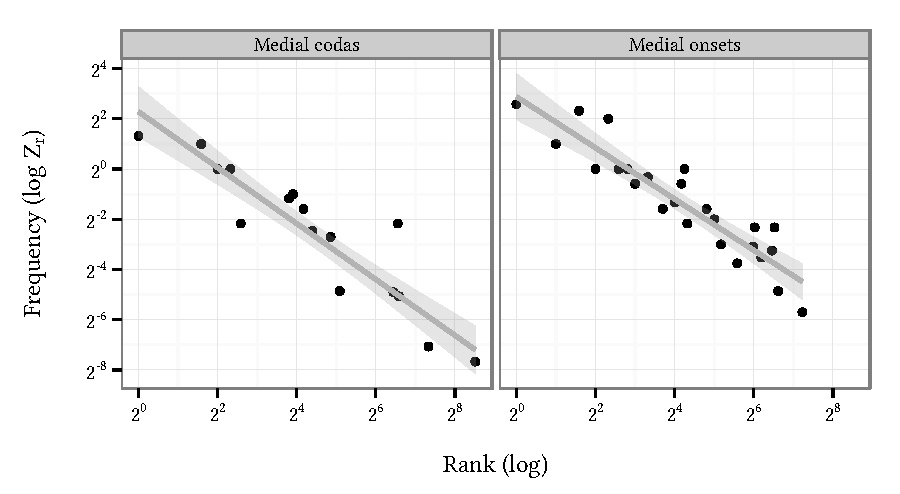
\includegraphics{co.pdf}
\caption{Medial coda and medial onset type frequencies in the lexical sample show a Zipfian distribution; frequencies have been smoothed using the $Z_r$ transform (see Appendix \ref{zr}).}
\label{cao}
\end{figure}

\begin{example}[Simulation procedure]
\begin{tabular}{l l}
a. & Sample a medial coda according to the observed probabilities  \\
b. & Sample a medial onset according to the observed probabilities \\
c. & Apply the \emph{SPE} rules to the cluster formed by their concatenation \\
\end{tabular}
\end{example}

This procedure corresponds to the assumption that the derived constraints impose the only structural restrictions on the cluster inventory.
Cluster frequencies in one simulated sample are shown in Figure \ref{sim}; dots represent simulated frequencies, and the line represents actual cluster frequencies.
As can be seen, the observed and simulated frequencies are quite similar 
($R^2 = 0.712$, $p = 4.5$\e{-05}).
The sparse cluster inventory, previously taken as evidence for static constraints on syllable contact clusters, is expected even if the only constraints on possible clusters are those which are phonologically derived.

\begin{figure}
\centering
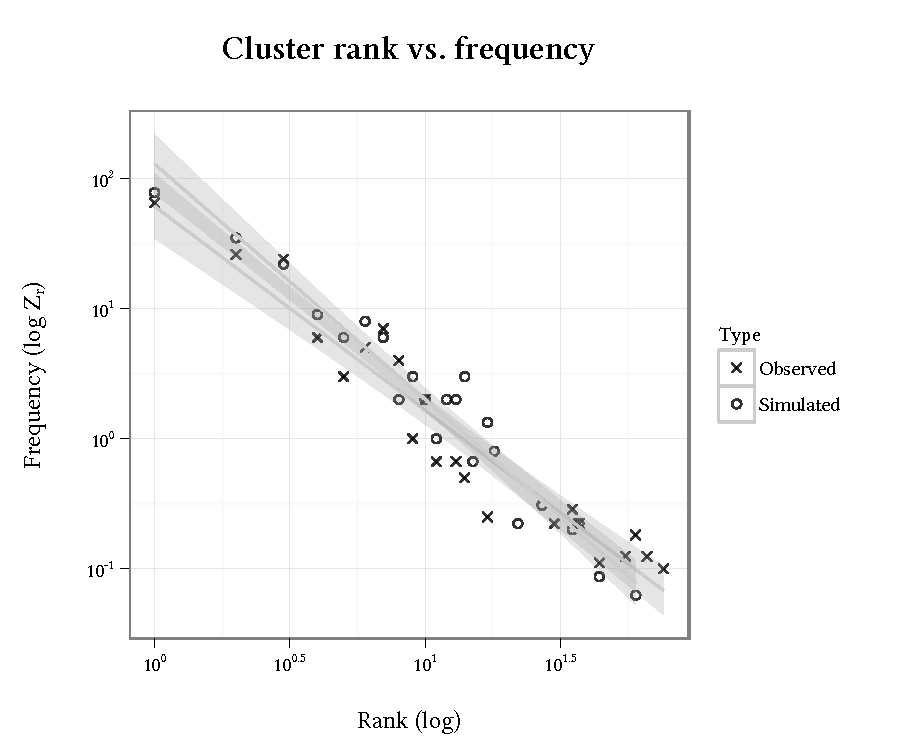
\includegraphics{sim.pdf}
\caption{A simulated cluster inventory, generated by random sampling and applying phonological neutralizations closely matches the observed cluster frequencies (represented by the smoothing line). Simulated and observed frequencies have been smoothed using the $Z_r$ transform (see Appendix \ref{zr}).}
\label{sim}
\end{figure}

\section{Conclusions}

The foregoing results demonstrate that the only structural constraints on English syllable contact are derived from the phonological system: there is no evidence for static constraints in this domain.
What then is to be said of the 366 clusters which do not violate a derived constraint, but which are yet unattested, like [b.z] or [z.n]? 
These gaps appear to be phonologically arbitrary, since they are not reliably identified either by phonologist or computional model.
They can only be understood as accidental gaps resulting from the sparsity of the sample and the finite nature of the English lexicon.

%It is quite apparent that root-internal hetero-voiced obstruent clusters like [s.b] or [z.t] are also rare compared to clusters which are uniformly voiced or uniformly voiceless, as predicted the assimilation rule. Yet, \citet{Pierrehumbert1994} does not mention voice assimilation in her study of English syllable contact clusters. \citet[][74f.]{Hammond1999a} cites words like \emph{a}[b.s]\emph{inth} and \emph{a}[s.b]\emph{estos}, which contain hetero-voiced obstruent clusters, as evidence that the process does not apply root-internally, though few of his examples are in fact simplex according to CELEX.\footnote{The \textsc{Revised Alternation Condition} (RAC) proposed by \citeauthor{Kiparsky1973a} (\citeyear{Kiparsky1973a}:163, \citeyear{Kiparsky1982a}:152) blocks the application of obligatory neutralization processes like \textsc{Obstruent Voice Assimilation} in root-internal (i.e., non-derived) environments. Simply because there are exceptions in non-derived environments, \textsc{Obstruent Voice Assimilation} is always consistent with the RAC whether or not it actually applies in non-derived environments. This is due to the ``obligatory'' condition of the RAC. If the rule applies in non-derived environments, then it has lexical exceptions (e.g., \emph{a}[s.b]\emph{estos}) and is not obligatory and thus free from the RAC. On the other hand, if the rule is subject to the RAC, it only applies in derived environments, in which it is obligatory.}
% 
%The question is: does \textsc{Obstruent Voice Assimilation} contribute a meaningful characterization the English lexicon? More specifically, are hetero-voiced clusters underrepresented in a way that is unlikely under the hypothesis of free combination? To answer this question, the 720 clusters in which both the final coda consonant and initial onset consonant are obstruent are sorted into four bins, according to whether they are attested or not, and whether or not the conform to the derived constraint---both obstruents are either voiced or voiceless, like in \emph{hu}[z.b]\emph{and} or \emph{rha}[p.s]\emph{osdy}, respectively---or violate it, like the aforementioned \emph{a}[b.s]\emph{inth} and \emph{a}[s.b]\emph{estos}. 

%\citet{McGowan2009} claims that the type frequency of individual syllable contact clusters in English is predicted by the change of sonority in the clusters.\footnote{Thanks to Maria Gouskova for bringing this study to my attention.} Using a sonority scale proposed by \citet{Jespersen1904}, \citeauthor{McGowan2009} reports that clusters like [m.p], with sharply falling sonority, are slightly more frequent than those like [t.j], with rising sonority. However, \citeauthor{McGowan2009} finds that sonority of clusters accounts for a very small of the variance in cluster frequency ($R^2 = 0.077$). As a predictor of cluster attestation, sonority distance provided no improvement over the null baseline; consequently, it is not included in Table \ref{cmresults}.
